\question Q2\droppoints

\begin{solution}
    \text{(a) - (f)} Implemented.

    \text{(g)} Using the \textbf{RandomizedSearchCV} class to set the range of hyperparameters and find the best hyperparameter combination.
    I set the number of iteration to $50$ and got the following hyperparameters:

    \begin{itemize}
        \item { $C = 2.087156815341724$ }
        \item { $\gamma = 0.006522117123602399$ }
        \item { kernel: RBF }
    \end{itemize}

    Use these hyperparameters to build the ``best classifier''.
    The following is the classification report of the ``best classifier'':

    \vspace{12pt}
    \centerline {
        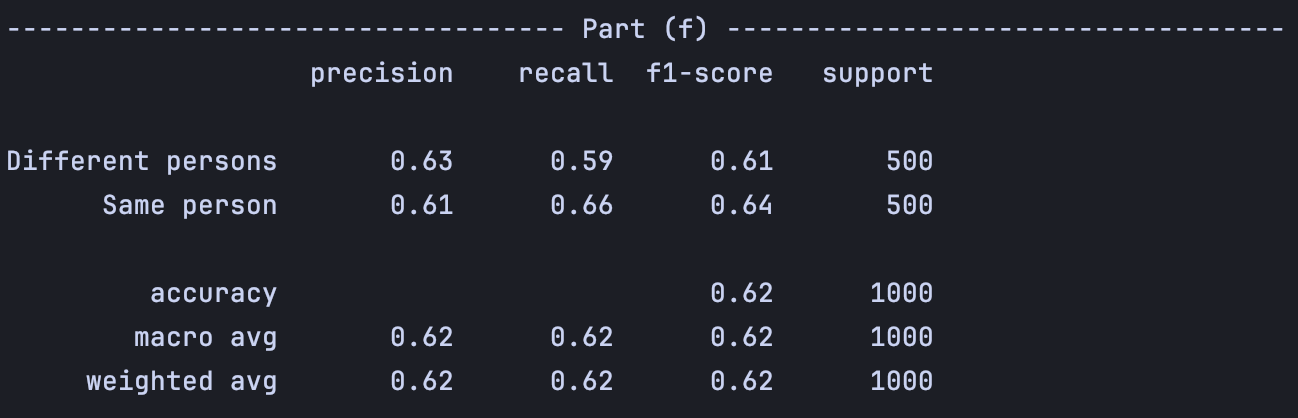
\includegraphics[width=0.75\textwidth]{img/q2_report}
    }

    And the confusion matrix is:

    \vspace{12pt}
    \centerline {
        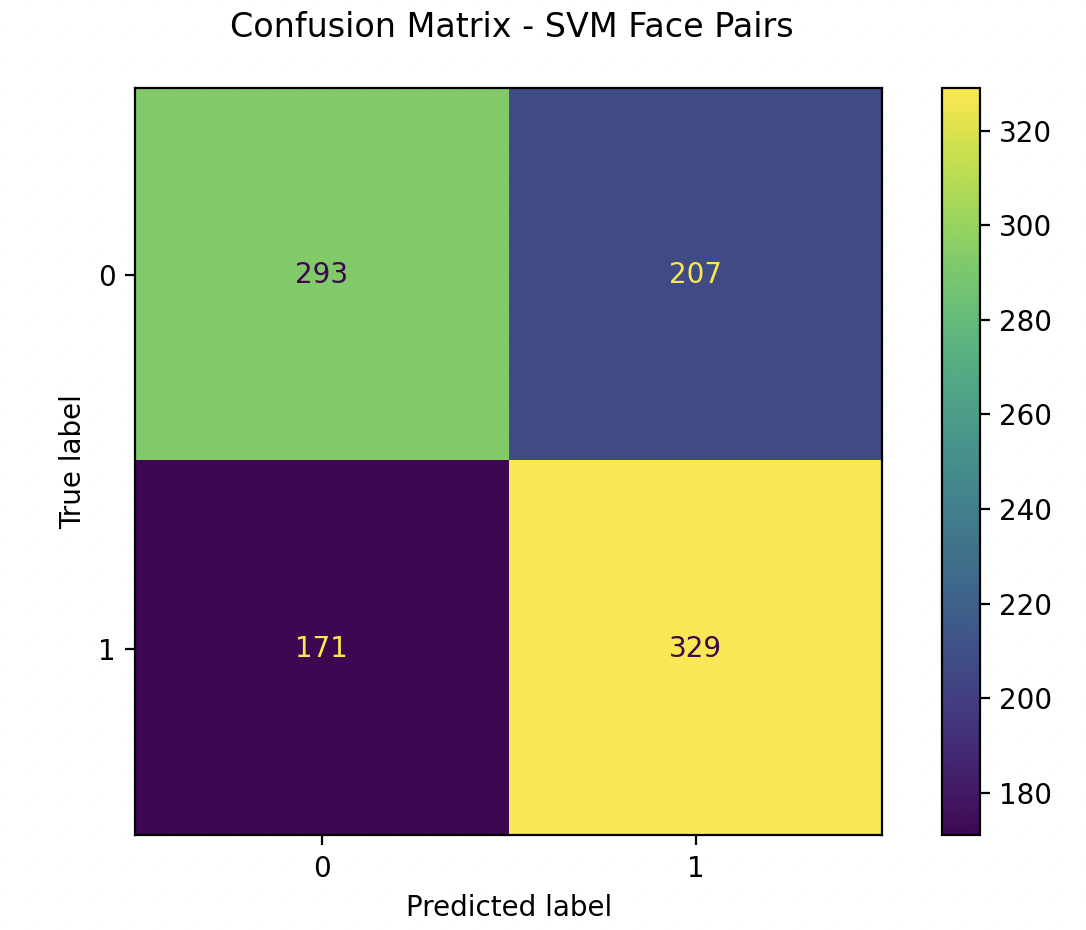
\includegraphics[width=0.75\textwidth]{img/q2_confusion_matrix}
    }

    The precision for both classes is around $0.61$ to $0.63$, indicating a balanced but moderate rate of correct positive predictions.
    The classifier is better at identifying ``Same person'' ($0.66$) than ``Different person'' ($0.59$).

    \text{(h)} To improve performance, I can:

    \begin{enumerate}
        \item { Increase the \textbf{n\_iter} in \textbf{RandomizedSearchCV}. }
        \item { Try different distributions in hyperparameter tuning. }
        \item { Use PCA for dimensionality reduction to reduce overfitting. }
    \end{enumerate}
\end{solution}